% !TeX root=../main.tex
\chapter{دانش پیش‌زمینه}
%\thispagestyle{empty} 
\section{مقدمه}
در این فصل مفاهیم مورد نیاز و استفاده در این پروژه مورد بررسی قرار می‌گیرند.
این فصل، محل شرح کامل روش تحقیق است و بسته به نوع روش تحقیق و با نظر استاد راهنما می‌تواند «مواد و روش‌ها%
\LTRfootnote{Materials and Methods}»
نیز نام بگیرد. این فصل حدود ۱۵ صفحه است.

\section{شبکه‌های مبتنی بر نرم‌افزار}

% \section{نت‌کت }
نت‌کت
،یک زبان برای توصیف شبکه‌های مبتنی بر نرم‌افزار است
\cite{netkat}.
این زبان با وجود دستور زبان
\lf{Syntax}
ساده‌ای که دارد، بر اساس
KAT
\cite{kat}
بنا شده و به همین دلیل یک سیستم معادلاتی صحیح و کامل
\lf{Sound and Complete}
دارد.
این سیستم معادلاتی کمک می‌کند تا با استفاده از روش‌های جبری و اثبات تساوی برنامه‌های توصیف شده در این زبان بتوان در مورد آن‌ها استدلال کرد.

\subsection{دستور زبان نت‌کت}
در نت‌کت هر بسته
به عنوان یک نگاشت از یک مجموعه از فیلد‌های
$f_1,f_2,...,f_n$
به اعداد طبیعی با تعداد ارقام ثابت در نظر گرفته می‌شود.
آی‌پی‌
\lf{IP}
های مبدا و مقصد، نوع بسته، پورت‌
\lf{Port}
های مبدا و مقصد مثال‌هایی از این فیلد‌ها هستند.
دستور زبان نت‌کت به صورت زیر تعریف می‌شود:
\begin{align*}
    a,b ::= & 1 | 0 | f = n | a + b | a \cdot b | \neg a  \\
    p,q ::= & a | f \la n | p + q | p \cdot q | p^* | dup
\end{align*}
در این گرامر عبارت‌های
$a,b$
عملا معادل با تست‌های زبان کت
\lf{KAT}
هستند.
عبارت‌های
$p,q$
عبارت‌های نت‌کت را تعریف می‌کنند که نسبت به دستور زبان کت
جمله‌هایی به شکل
$dup$
و
$f \la n$
به آن اضافه شده است.
\subsection{مدل معنایی نت‌کت}
برای اینکه امکان استدلال در مورد مسیر‌های طی شده توسط یک بسته‌ در شبکه وجود داشته باشد،از مفهومی به نام تاریخچه‌ی بسته
\lf{Packet History}
استفاده می‌شود.
هر تاریخچه‌ی بسته‌، یک دنباله از بسته‌ها است که بسته نخست دنباله، به عنوان بسته‌ی فعلی در نظر گرفته می‌شود.
به صورت شهودی
عبارت های ۱ و ۰ به ترتیب به معنای ارسال
\lf{Forward}
و رها کردن
\lf{Drop}
بدون شرط بسته هستند.
عبارت
$f=n$
در صورتی بسته را عبور می‌دهد که مقدار فیلد
f
آن برابر با
n
باشد.
عبارت
$f \la n$
مقدار n
را به فیلد f
بسته اختصاص
می‌دهد.
عبارت‌های
$dup$
باعث می‌شوند تا یک کپی از بسته‌ی فعلی ایجاد شود و به تاریخچه‌ی بسته‌ها اضافه شود.
این عبارات در رفتار شبکه تاثیری ندارند اما امکان استدلال در مورد تمامی تغییرات ایجاد شده در حین جا‌به‌جایی بسته در شبکه را فراهم می‌سازند.
به صورت دقیق، معنای هر عبارت
\lf{Expression}
نت‌کت با استفاده از معادلات زیر تعریف می‌شود:
\begin{align}
    \sem{p}             & H \in \mathcal{P}({H}) \label{eq:netkat:sem}                  \\
    \sem{1} h           & \teq \s{h}     \label{eq:netkat:identity}                     \\
    \sem{0} h           & \teq \s{}          \label{eq:netkat:drop}                     \\
    \sem{f=n}(pk::h)    & \teq \begin{cases}
                                   \s{pk::h} & \text{ if } pk.f = n \\
                                   \s{}      & \text{ otherwise }
                               \end{cases}    \label{eq:netkat:filter}                  \\
    \sem{\neg a}        & \teq \s{h} \setminus (\sem{a}h) \label{eq:netkat:nfilter}     \\
    \s{f \la n} (pk::h) & \teq \s{pk[f:=n]::h}     \label{eq:netkat:assign}             \\
    \sem{p+q}h          & \teq \sem{p}h \cup \sem{q}h   \label{eq:netkat:sum}           \\
    \sem{p\cdot q} h    & \teq (\sem{p} \bullet \sem{q}) h    \label{eq:netkat:dot}     \\
    \sem{p^*}h          & \teq \bigcup_{i \in \mathbb{N}}F^i h \label{eq:netkat:kleene} \\
    F^0 h               & \teq \s{h}                                                    \\
    F^{i+1} h           & \teq (\sem{p} \bullet F^i) h                                  \\
    (f \bullet g) x     & \teq \bigcup\s{g(y)|y \in f(x)}                               \\
    \sem{dup} (pk::h)   & \teq \s{pk::(pk::h)} \label{eq:netkat:dup}
\end{align}
در معادلات بالا فرض می‌شود که 
$H$
مجموعه‌ی تمامی تاریخچه‌های ممکن است.
معادله‌ی 
\ref{eq:netkat:sem}
بیان می‌کند که معنی هر عبارت نت‌کت روی یک تاریخچه‌ی بسته یک مجموعه از  
تاریخچه‌ی بسته‌های حاصل از اعمال این عبارت روی تاریخچه‌ی ورودی است.
معادله‌ی 
\ref{eq:netkat:identity}
بیان می‌کند که عبارت ۱ بسته را بدون شرط عبور می‌دهد.
در مقابل معادله‌ی 
\ref{eq:netkat:drop}
رها شدن بسته را با خروجی یک مجموعه‌ی خالی مدل می‌کند.
معادله‌ی 
\ref{eq:netkat:filter}
بسته‌ی نخست ورودی را بررسی می‌کند و اگر مطابق با عبارت نبود بسته رها می‌شود.
معادله‌ی
\ref{eq:netkat:assign}
مقدار 
$n$
را به فیلد
$f$
بسته‌ی نخست تاریخچه اختصاص می‌دهد.
در معادله‌ی 
\ref{eq:netkat:kleene}
حاصل اپراتور ستاره‌ی کلین
\lf{Kleene Star}
معادل با اجتماع اعمال عبارت به تعداد دلخواه روی تاریخچه‌ی ورودی در نظر گرفته شده است.
در نهایت معادله‌ی 
\ref{eq:netkat:dup}
یک کپی از بسته‌ی نخست ورودی را به ابتدای خروجی اضافه می‌کند.

نت‌کت علاوه بر اصول موضوعه‌ی
\lf{Axiom}
KAT
اصول‌ موضوعه‌ی زیر را هم شامل می‌شود تا دستگاه معادلاتی صحیح و کامل
\lf{Sound and Complete}
داشته باشد:
\begin{align}
    f \la n \cdot f' \la n' & \equiv f' \la n' \cdot f \la n,
    \text{ if } f \neq f' \label{mod-mod-comm}
    \\
    f \la n \cdot f' = n'   & \equiv f' = n' \cdot f \la n,
    \text{ if } f \neq f' \label{mod-filter-comm}                            \\
    dup \cdot f = n         & \equiv f = n \cdot dup \label{dup-filter-comm} \\
    f \la n \cdot f = n     & \equiv f \la n \label{mod-filter}              \\
    f = n \cdot f \la n     & \equiv f = n \label{filter-mod}                \\
    f \la n \cdot f \la n'  & \equiv f \la n' \label{mod-mod}                \\
    f = n \cdot f = n'      & \equiv 0, \text{ if } n \neq n' \label{contra} \\
    \Sigma_{i} f = i        & \equiv 1 \label{match-all}
\end{align}
اصل‌های
\ref{mod-mod-comm},\ref{mod-filter-comm},\ref{dup-filter-comm}
خواص جابه‌جایی
\lf{Commutative}
عملیات‌ها را بیان می‌کنند.
اصل
\ref{mod-filter}
بیان می‌کند که اختصاص مقدار
n
به یک فیلد و سپس  فیلتر کردن بر روی این فیلد با همین مقدار معادل با عملیات اختصاص
\lf{Assignment}
به تنهایی است.
مشابه همین اصل برای یک فیلتر و سپس یک اختصاص هم در اصل
\ref{filter-mod}
مشخص شده.
اصل
\ref{mod-mod}
بیان می‌کند که در دنباله‌ای از اختصاص مقادیر به یک فیلد مشخص، تنها آخرین اختصاص تاثیر دارد.
در اصل
\ref{contra}
مشخص شده است که مقدار یک فیلد نمی‌تواند دو مقدار متفاوت داشته باشد.
در نهایت اصل
\ref{match-all}
بیان می‌کند که عملیات مجموع فیلتر‌ها به ازای هر مقدار ممکن برای یک فیلد مشخص برابر عنصر همانی
\lf{Identity}
است.

\subsection{توصیف رفتار شبکه با نت‌کت}

در ادامه نحوه‌ی توصیف یک شبکه با استفاده از نت‌کت بیان می‌شود.
\begin{figure}
    \centering
    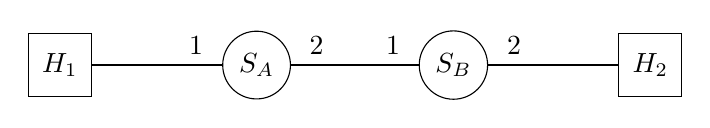
\begin{tikzpicture}[
            node distance={25mm},
            sw/.style = {draw, circle,minimum size=8mm},
            h/.style = {draw, rectangle,minimum size=8mm}
        ]
        \node[h] (h1)  {$H_1$};
        \node[sw] (sa) [right of=h1]  {$S_A$};
        \node[sw] (sb) [right of=sa] {$S_B$};
        \node[h] (h2)  [right of=sb] {$H_2$};
        \draw [thick] (h1)  -- node[above,pos=0.8]{1} (sa);
        \draw [thick] (sa) -- node[above,pos=0.2]{2}
        node[above,pos=0.8]{1}(sb);
        \draw [thick] (sb) -- node[above,pos=0.2]{2} (h2);
    \end{tikzpicture}
    \caption{مثال شبکه}
    \label{fig:netkat:ssh}
\end{figure}
در شکل
\ref{fig:netkat:ssh}
شبکه شامل دو سوییچ
\lf{Switch}
A و ‌B
و دو هاست
\lf{Host}
می‌باشد.
هر سوییچ دو پورت دارد که با شماره‌های ۱ و۲ مشخص شده‌اند.
در این شبکه هدف این است که امکان جا‌به‌جایی همه‌ی بسته‌ها به غیر از بسته‌هایی که از نوع
SSH
هستند وجود داشته باشد.
عبارت نت‌کت زیر را در نظر بگیرید:
\begin{align*}
    p \triangleq (dst = H_1 \cdot pt \la 1) +
    (dst = H_2 \cdot pt \la 2)
\end{align*}
این عبارت همه‌ی بسته‌هایی که مقصد آن‌ها هاست ۱ باشد را به پورت ۱ و همه‌ی بسته‌هایی که مقصد‌ آن‌ها هاست ۲ باشد را به پورت شماره‌ی ۲ می‌فرستد.
این سیاست
\lf{Policy}
به سادگی رفتار سوییچ‌ها را در نت‌کت تعریف می‌کند.
در ادامه می‌توان با اضافه کردن یک فیلتر به این عبارت، ویژگی دسترسی کنترل
\lf{Access Control}
را به این سیاست اضافه کرد تا همه‌ی بسته‌های از نوع
SSH
رها شوند:
\begin{align*}
    p_{AC} \triangleq \neg(typ = SSH)\cdot p
\end{align*}
اما استفاده از عبارت بالا به تنهایی برای توصیف رفتار شبکه شکل
\ref{fig:netkat:ssh}
کافی‌ نیست.
برای تکمیل این عبارت لازم است تا رفتار توپولوژی
\lf{Topology}
شبکه‌ هم به آن افزوده شود.
در نت‌کت توپولوژی شبکه به عنوان یک گراف جهت‌دار در نظر گرفته می‌شود و رفتار آن در قالب اجتماع رفتار هر یک از پیوندهای
\lf{Link}
آن توصیف می‌شود.
برای شبکه‌ی شکل
\ref{fig:netkat:ssh}
می‌توان از عبارت زیر برای توصیف توپولوژی شبکه استفاده کرد:
\begin{align*}
    t \triangleq & (sw = A \cdot pt = 2 \cdot sw \la B \cdot pt \la 1) + \\
                 & (sw = b \cdot pt = 1 \cdot sw \la A \cdot pt \la 2) + \\
                 & (sw = b \cdot pt = 2)
\end{align*}
در نت‌کت در صورتی که سیاست و توپولوژی شبکه در قالب عبارت‌هایی توصیف شده‌باشند،
رفتار کل شبکه در واقع دنباله‌ای از اعمال این عبارت‌ها به صورت یکی در میان است.
به عنوان مثال در شکل
\ref{fig:netkat:ssh}
یک بسته از هاست ۱ ابتدا توسط سوییچ
A
پردازش شده، سپس روی لینک بین دو سوییچ جا به جا می‌شود و در نهایت توسط سوییچ
B
پردازش می‌شود.
در نت‌کت می‌توان این رفتار را به صورت
$p_{AC}\cdot t \cdot p_{AC}$
توصیف کرد.
با استفاده از همین شهود، رفتار کل شبکه را می‌توان در قالب عبارت زیر توصیف کرد:
\begin{align*}
    (p_{AC}\cdot t)^*
\end{align*}
در توصیف بالا فرض شده است که بسته‌ها می‌توانند به هر طریق ممکن وارد شبکه و از آن خارج شوند، اما این رفتار همیشه مورد قبول نیست.
به عنوان مثال در شبکه شکل
\ref{fig:netkat:ssh}
اگر مکان‌های ورودی و خروجی شبکه را در قالب عبارت زیر توصیف کنیم:
\begin{align*}
    e \triangleq sw = A\cdot port = 1 \vee sw = B \cdot port = 2
\end{align*}
می‌توانیم رفتار انتها به انتهای
\lf{End to End}
شبکه را به شکل زیر توصیف کنیم:
\begin{align*}
    p_{net} \triangleq e \cdot (p_{AC}\cdot t)^* e
\end{align*}
در حالت کلی‌تر، نیازی به توصیف ورودی و خروجی‌های شبکه در قالب یک عبارت نیست.
پس اگر فرض شود که مکان‌های ورودی شبکه توسط عبارت
$in$
و مکان‌های خروجی شبکه در قالب عبارت
$out$
توصیف شده‌ باشند، رفتار یک شبکه در نت‌کت به صورت زیر تعریف می‌شود:
\begin{align*}
    in \cdot (p\cdot t)^*\cdot out
\end{align*}
که عبارت
$p$
سیاست شبکه و عبارت
$t$
توپولوژی شبکه است.

\subsection{درستی‌سنجی برنامه‌های نت‌کت}
درستی‌سنجی یک شبکه و بررسی خواص آن در نت‌کت با استفاده از بررسی تساوی عبارت یک شبکه با عبارت‌های دیگر انجام می‌شود.
به عنوان مثال در شبکه‌ی شکل
\ref{fig:netkat:ssh}
برای بررسی اینکه همه‌ی بسته‌ها با نوع
SSH
از هاست ۱ رها می‌شوند کافی است تا تساوی زیر را ثابت کنیم:
\begin{equation*}
    \begin{pmatrix}
        type = SSH \cdot sw = A \cdot pt = 1 \cdot \\
        (p_{AC}\cdot t) ^ * \cdot                  \\
        sw = B\cdot pt = 2
    \end{pmatrix}
    \equiv 0
\end{equation*}
از طرفی برای بررسی یک خاصیت در شبکه، مثلا امکان فرستاده شدن‌ همه‌ی بسته‌هایی که از نوع
SSH
نیستند از هاست ۱ به هاست ۲
می‌توان به جای بررسی تساوی دو عبارت از نامساوی
$p \leq q$
استفاده کرد.
این نامساوی که خلاصه شده‌ی تساوی
$p + q \equiv q$
است بیان می‌کند که رفتار عبارت
$p$
بخشی از رفتار عبارت
$q$
است.
بنابراین برای بررسی این مساله که شبکه‌ی شکل
\ref{fig:netkat:ssh}
بسته‌های غیر
$SSH$
از هاست ۱ را عبور می‌دهد کافی است تا درستی نامعادله‌ی زیر را بررسی کرد:
\begin{equation*}
    \begin{pmatrix}
        \neg(type = SSH) \cdot sw = A \cdot pt = 1 \cdot & \\
        sw \la B \cdot pt \la 2                          &
    \end{pmatrix}
    \leq (p_{AC}\cdot t)^ *
\end{equation*}

% \section{نت‌کت پویا}
نک‌کت‌ پویا
\lf{DyNetKAT}
برای رفع برخی از کاستی‌های نت‌کت ارائه شده است
\cite{dynetkat}.
به صورت دقیق‌تر نت‌کت پویا، امکان توصیف به‌روز‌رسانی سیاست‌های شبکه و همچنین رفتار شبکه در مقابل چندین بسته را ممکن می‌سازد.

\subsection{دستور زبان نت‌کت پویا}
در نت‌کت‌ پویا، از رفتار انتها به انتها‌ی توصیف‌های شبکه در قالب عبارت‌های نت‌کت استفاده می‌شود.
به همین منظور سینتکس نت‌کت‌ پویا به صورت زیر تعریف می‌شود:
\begin{align*}
    N & :: = \mathrm{NetKAT}^{-dup}                    \\
    D & :: = \bot | N;D | x?N;D | x!N;D | D\parallel D
    D \oplus D | X                                     \\
      & X \triangleq D
\end{align*}
در سینتکس بالا
$\mathrm{NetKAT}^{-dup}$
قسمتی از زبان نت‌کت است که عبارت‌های
$dup$
از آن حذف شده است.
عبارت‌های
$dup$
در توصیف‌های نت‌کت تاثیری در رفتار یک عبارت ندارند و هدف از استفاده از آن‌ها ثبت یک اثر از هر بسته پس از پردازش توسط یکی از عناصر شبکه است و امکان استدلال بر روی رفتار شبکه را ممکن می‌سازد.
با توجه به این که در نت‌کت پویا رفتار انتها به انتهای یک عبارت نت‌کت مورد استفاده است، عبارت
$dup$
از دستور زبان کنار گذاشته شده است.
نت‌کت‌پویا یک لیست از بسته‌های ورودی را پردازش می‌کند و یک لیست از مجموعه‌ی بسته‌های خروجی تولید می‌کند.
اپراتور ترکیب متوالی
\lf{Sequential Composition}
$N;D$
باعث می‌شود که یک بسته از لیست بسته‌های ورودی توسط سیاست
$N$
پردازش شود و سپس بسته‌ی توسط عبارت
$D$
پردازش می‌شود.
در نت‌کت پویا امکان ارتباط توسط عبارت‌هایی به شکل
$x!N$
و
$x?N$
توصیف می‌شوند که به ترتیب ارسال و دریافت یک عبارت نت‌کت را روی کانال
$x$
توصیف می‌کنند.
ترکیب موازی
\lf{Parallel Composition}
دو عبارت توسط
$D \parallel D$
توصیف می‌شود.
در نهایت رفتار‌های غیرقطعی
\lf{Non-Deterministic}
توسط‌ عبارت‌هایی به شکل
$D \oplus D$
توصیف می‌شوند.

\subsection{معنای عملیاتی نت‌کت پویا}
معنای عملیاتی
\lf{Operational Seamntic}
نت‌کت پویا با استفاده از عبارت‌هایی به شکل
$(d,H,H')$
تعریف می‌شوند که
$d$
عبارت نت‌کت‌ پویا فعلی است،
$H$
لیست بسته‌هایی که در ادامه باید پردازش شوند
و
$H'$
لیست بسته‌هایی است که به صورت موفقیت‌آمیز توسط شبکه پردازش شده‌اند.
در اینجا فرض می شود که
$F = \s{f_1,...,f_n}$
یک مجموعه از فیلد‌های بسته‌ها است.
یک بسته به شکل یک تابع
$F \ra \mathbb{N}$
توصیف می‌شود.
برای یک بسته مانند
$\sigma$
تساوی
$\sigma(f_i) = v_i$
بیان می‌کند که مقدار فیلد
$f_i$
در بسته‌ی
$\sigma$
برابر با
$v_i$
است.
یک لیست خالی از بسته‌ها با
$\his{}$
نمایش داده می‌شود.
اگر
$l$
یک لیست از بسته‌ها باشد
$e::l$
لیستی است که حاصل از اضافه کردن بسته
$\sigma$
به ابتدای لیست به دست می‌آید.
برچسب هر قانون که با
$\gamma$
مشخص می‌شود به صورت یکی از شکل‌های
$(\sigma,\sigma'),x!q,x?q$
یا
$rcfg(x,q)$
تعریف می‌شود
که
$rcfg(x,q)$
به معنی انجام شدن
$x!q$
و
$x?q$
به صورت همگام
\lf{Synchronized}
است.
قوانین زیر معنای عملیاتی نت‌کت پویا را تعریف می‌کنند:
\begin{align}
     & (cpol^{\checkmark}_{\_;})
    \frac{\sigma' \in \sem{p}(\sigma::\his{})}
    {(p;q,\sigma::H,H')\xrightarrow{(\sigma,\sigma')}
    (q,H,\sigma'::H') }    \label{os:term}                                 \\
     & (cpol_X)
    \frac{(p,H_0,H_1)\xrightarrow{\gamma}(p',H_0',H_1')}
    {(X,H_0,H_1)\xrightarrow{\gamma}(p',H_0',H_1')}
    X \triangleq p         \label{os:recr}                                 \\
     & (cpol_{\_\oplus})
    \frac{(p,H_0,H_0')\xrightarrow{\gamma}(p',H_1,H_1')}
    {(p\oplus q,H_0,H_0')\xrightarrow{\gamma}(p',H_1,H_1')}
    \label{os:orr}                                                         \\
     & (cpol_{\oplus\_})
    \frac{(q,H_0,H_0')\xrightarrow{\gamma}(q',H_1,H_1')}
    {(p\oplus q,H_0,H_0')\xrightarrow{\gamma}(p',H_1,H_1')} \label{os:orl} \\
     & (cpol_{\_\parallel})
    \frac{(p,H_0,H_0')\xrightarrow{\gamma}(p',H_1,H_1')}
    {(p\parallel q,H_0,H_0')\xrightarrow{\gamma}(p' \parallel q,H_1,H_1')}
    \label{os:parr}                                                        \\
     & (cpol_{\parallel\_})
    \frac{(q,H_0,H_0')\xrightarrow{\gamma}(q',H_1,H_1')}
    {(p\parallel q,H_0,H_0')\xrightarrow{\gamma}(p \parallel q',H_1,H_1')}
    \label{os:parl}                                                        \\
     & (cpol_?)
    \frac{}
    {(x?p;q,H,H')\xrightarrow{x?p}(q,H,H')}
    \label{os:recv}                                                        \\
     & (cpol_!)
    \frac{}
    {(x!p;q,H,H')\xrightarrow{x!p}(q,H,H')}
    \label{os:send}                                                        \\
     & (cpol_{!?})
    \frac{
        (q,H,H') \xrightarrow{x!p}(q',H,H')
        (s,H,H') \xrightarrow{x?p} (s',H,H')
    }{
        (q\parallel,H,H') \xrightarrow{rcfg(x,p)} (q'\parallel s',H,H')
    }     \label{os:syncr}                                                 \\
     & (cpol_{?!})
    \frac{
        (q,H,H') \xrightarrow{x?p}(q',H,H')
        (s,H,H') \xrightarrow{x!p} (s',H,H')
    }{
        (q\parallel,H,H') \xrightarrow{rcfg(x,p)} (q'\parallel s',H,H')
    } \label{os:syncl}
\end{align}
قانون 
\ref{os:term}
انجام یک عملیات مانند
$(\sigma,\sigma')$
که به معنای
پردازش بسته‌ی ابتدایی لیست ورودی توسط عبارت 
$p$
و افزودن خروجی حاصل از آن مانند 
$\sigma'$
به لیست خروجی است را مشخص می‌کند.
قانون 
\ref{os:recr}
بیان می‌کند که رفتار متغیر 
$X$
که برابر با عبارت 
$p$
است معادل با رفتار عبارت 
$p$
است.
قوانین 
\ref{os:orr}
و
\ref{os:orl}
رفتار غیرقطعی را توصیف می‌کنند.
قوانین
\ref{os:parr}
و
\ref{os:parl}
رفتار دو عبارت موازی را توصیف می‌کنند.
قوانین
\ref{os:recv}
و
\ref{os:send}
مشخص می‌کنند که ارسال یا دریافت پیام در نت‌کت پویا پردازشی روی بسته‌ها انجام نمی‌دهد.
در نهایت همگام‌سازی
\lf{Synchronization}
ارسال و دریافت پیام توسط قوانین 
\ref{os:recv}
و
\ref{os:send}
توصیف شده است.

\subsection{توصیف برنامه‌ها در نت‌کت پویا}

\begin{figure}
    \centering
    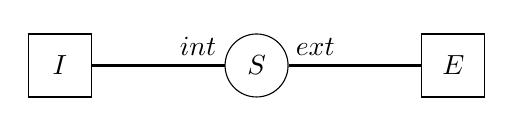
\begin{tikzpicture}[
            node distance={25mm},
            sw/.style = {draw, circle,minimum size=8mm},
            h/.style = {draw, rectangle,minimum size=8mm}
        ]
        \node[h] (i)  {$I$};
        \node[sw] (s) [right of=i]  {$S$};
        \node[h] (e)  [right of=s] {$E$};
        \draw [thick] (i)  -- node[above,pos=0.8]{$int$} (s);
        \draw [thick] (s) -- node[above,pos=0.2]{$ext$} (e);
    \end{tikzpicture}
    \caption{مثال دیوار آتش}
    \label{fig:dynetkat:firewall}
\end{figure}
در ادامه چگونگی توصیف یک دیوار آتش
\lf{Firewall}
وابسته به حالت
\lf{Stateful}
با استفاده از نت‌کت پویا بیان می‌شود.
شبکه‌ی شکل
\ref{fig:dynetkat:firewall}
را در نظر بگیرید.
در این شبکه هدف این است که امکان ارتباط از داخل شبکه به بیرون فراهم باشد ولی امکان ارسال بسته از خارج شبکه ممکن نباشد.
اما زمانی که یک بسته به خارج شبکه ارسال شد، دیوار آتش باید اجازه‌ی عبور بسته‌ها از بیرون را بدهد تا پاسخ بسته‌ها دریافت شوند.
برای توصیف این شبکه می‌توان از عبارت نت‌کت پویای زیر استفاده کرد:
\begin{align*}
    Host  \triangleq   & secConReq!1;Host \oplus secConEnd!1;Host        \\
    Switch \triangleq  & (port = int) \cdot (port \la ext);Switch \oplus \\
                       & (port = ext)\cdot 0 ; Switch \oplus             \\
                       & secConReq?1;Switch'                             \\
    Switch' \triangleq & (port =int) \cdot (port \la ext);Switch' \oplus \\
                       & (port=ext)\cdot(port\la int);Switch' \oplus     \\
                       & secConEnd?1;Switch                              \\
    Init \triangleq    & Host \parallel Switch
\end{align*}
در این توصیف عملیات 
$secConReq$
برای شروع ارتباط امن و
$secConEnd$
برای خاتمه‌ی ارتباط امن در نظر گرفته شده‌است.
بنابراین برنامه‌ی سوییچ پس از دریافت پیام برای شروع ارتباط امن تبدیل به برنامه‌ی 
$Switch'$
می‌شود که در آن اجازه‌ی ارسال بسته از پورت خارجی به پورت داخلی را دارد.
پس از دریافت پیام برای خاتمه‌ی ارتباط امن، برنامه به حالت اولیه‌ی خود بر می‌گردد و دوباره تمامی بسته‌های ورودی از پورت خارجی را رها می‌کند.
در نهایت رفتار کل شبکه با استفاده از ترکیب موازی یک هاست و یک سوییچ در حالت اولیه خود توصیف می‌شود.
\begin{figure}[ht]
    \centerline{\includegraphics[width=0.8\textwidth]{mine/firewall-lts.png}}
    \caption{سیستم انتقال برچسب‌دار برای شبکه‌ی دیوار آتش}
    \label{fig:dynetkat:lts}
\end{figure}
نمودار نمایش داده شده در شکل
\ref{fig:dynetkat:lts}
سیستم انتقال برچسب‌دار
\lf{Labeled Transition System}
این شبکه‌ را در حالتی که یک بسته روی پورت ورودی و یک بسته روی پورت خروجی شبکه وجود دارد نشان می‌دهد.
همانطور که در نمودار مشخص است، عملیات
$(\sigma_e,\sigma_i)$
که به معنای ارسال بسته از پورت ورودی به پورت خروجی است تنها در قسمتی از این سیستم انتقال قابل دسترسی است که پیش از آن یکی از عملیات‌های
$SCR?1$
یا
$rcfg(SCR,1)$
انجام شده باشند.
بنابراین در این حالت شبکه تنها در صورتی که بسته خارجی را به داخل ارسال می‌کند که پیش از آن پیام آغاز ارتباط امن دریافت کرده‌ باشد.


\section{ساختمان رویداد}
ساختمان رویداد
\lf{Event Structure}
\cite{es}
یک مدل محاسباتی
\lf{Computational Model}
غیر‌جای‌گذاری شده
\lf{Non-Interleaving}
برای پردازه‌های هم‌روند
\lf{Concurrent}
است.
در این مدل، برخلاف مدل‌های جایگذاری شده
\lf{Interleaving}
مانند سیستم‌انتقال که هم‌روندی پردازه‌های موازی با انتخاب غیرقطعی مدل می‌شود، هم‌روندی پردازه‌ها به صورت صریح در مدل توصیف می‌شوند
\cite{sassone1996models}.
\begin{definition}{ساختمان رویداد}
    یک ساختمان رویداد یک سه‌تایی
    $(E,\#,\vdash)$
    است که در آن:
    \begin{enumerate}
        \item $E$
              یک مجموعه از رویداد‌ها است
        \item $\#$
              رابطه‌ی تعارض
              \lf{Conflict}
              ، یک رابطه‌ی دودویی متقارن و غیربازتابی بر روی مجموعه‌ی
              $E$
              است
        \item $\vdash \subseteq Con \times E$
              رابطه‌ی فعال سازی
              \lf{Enabling}
              است که شرط زیر را برقرار می‌کند:
              \begin{align*}
                  X \vdash e \wedge X \subseteq Y \in Con
                  \Rightarrow Y \vdash e
              \end{align*}
    \end{enumerate}
    در رابطه‌ی بالا
    $Con$
    زیرمجموعه‌ای از مجموعه‌ی توانی رویدادها است که اعضای آن فاقد تعارض باشند.
    به صورت دقیق‌تر داریم:
    \begin{align*}
        Con = \s{X \subseteq E| \forall e,e' \in X. \neg(e\#e')}
    \end{align*}
\end{definition}
\begin{definition}
    به ازای هر ساختمان رویداد، می‌توانیم رابطه‌ی فعال‌سازی مینیمال را به صورت زیر تعریف کنیم:
    \begin{align*}
        X \vdash_{min} e \iff X \vdash e \wedge
        ( \forall Y \subseteq X . Y \vdash e \Rightarrow Y = X )
    \end{align*}
    همچنین در هر ساختمان رویدادی شرط زیر برقرار است:
    \begin{align*}
        Y \vdash e \Rightarrow \exists X \subseteq Y . X \vdash_{min} e
    \end{align*}
\end{definition}

برای مشخص کردن وضعیت یک سیستم در هر لحظه از مفهومی به نام پیکر‌بندی
\lf{Configuration}
استفاده می‌شود و
و یک مجموعه شامل رویدادهایی است که تا آن لحظه در سیستم رخ داده‌اند.
\begin{definition}
    اگر
    $\mathrm{E} = (E,\#,\vdash)$
    یک ساختمان رویداد باشد، یک پیکربندی آن یک زیرمجموعه از رویداد‌ها
    $x \subseteq E$
    است که شرایط زیر را داشته باشد:
    \begin{enumerate}
        \item $x \in Con$
        \item $\forall e \in x \exists e_0,...,e_n \in x. e_n = e \ \&
                  \forall i \leq n. \s{e_0,...,e_{i-1}} \vdash e_i$
    \end{enumerate}
\end{definition}
مجموعه‌ی همه‌ی پیکربندی‌های یک ساختمان رویداد مانند
$\mathrm{E}$
با
$\mathcal{F}(\mathrm{E})$
نمایش داده می‌شود.

شبکه‌ی موجود در شکل
\ref{fig:es:update}
را در نظر بگیرید.
در این شبکه دو میزبان ۱ و ۲ به صورت هم‌روند یک بسته را به سوییچ ارسال می‌کنند.
این بسته‌ها شامل اطلاعات برای به روزرسانی مسیر‌های دیگر در شبکه هستند، بنابراین سوییچ پس از دریافت هر دوی این بسته‌ها آن ها را پردازش کرده و مسیر‌های خود را به روزرسانی می‌کند.
برای مدل کردن این شبکه می‌توانیم از یک ساختمان رویداد به صورت زیر استفاده کنیم:
\begin{align*}
    \mathrm{E} & = (
    \s{r_1,r_2,u},
    \e, \s{(\e,r_1),(\e,r_2),(\s{r_1,r_2},u)}
    )
\end{align*}
در این ساختمان رویداد، رویداد‌ها به ترتیب دریافت یک بسته از میزبان ۱، دریافت یک بسته از میزبان ۲ و به روز رسانی سوییچ را مدل می‌کنند.
یکی از روش‌های رسم نمودار برای ساختمان رویداد، رسم نمودار هس
\lf{Hasse}
برای مجموعه‌ی پیکربندی‌های این ساختمان رویداد بر اساس رابطه‌ی زیرمجموعه است.
برای مثالی که بیان شد می‌توان نموداری مطابق شکل
\ref{fig:es:configs}
را رسم کرد.
\begin{figure}
    \centering
    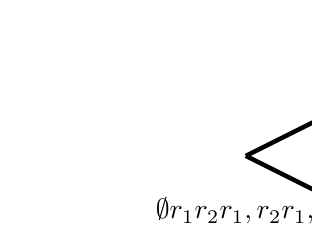
\begin{tikzpicture}[scale=0.8]
        \crd{0}{0}{$\emptyset$}
        \crd[left]{-2}{1}{$\s{r_1}$}
        \crd[right]{2}{1}{$\s{r_2}$}
        \crd[right]{0}{2}{$\s{r_1,r_2}$}
        \crd[right]{0}{3}{$\s{r_1,r_2,u}$}
        \draw [ultra thick] (0,0) -- (2,1);
        \draw [ultra thick] (0,0) -- (-2,1);
        \draw [ultra thick] (-2,1) -- (0,2);
        \draw [ultra thick] (2,1) -- (0,2);
        \draw [ultra thick] (0,2) -- (0,3);
    \end{tikzpicture}
    \caption{}
    \label{fig:es:configs}
\end{figure}

\begin{figure}
    \centering
    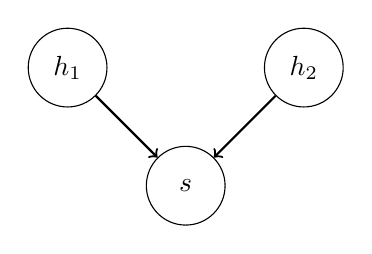
\begin{tikzpicture}[node distance={15mm},minimum size=10mm,
            main/.style = {draw, circle}]
        \node[main] (S)  {$s$};
        \node[main] (H1) [above of=S,left of=S] {$h_1$};
        \node[main] (H2) [above of=S,right of=S] {$h_2$};
        \draw[->,thick] (H1) -- (S);
        \draw[<-,thick] (S) -- (H2);
    \end{tikzpicture}
    \caption{}
    \label{fig:es:update}
\end{figure}
